\begin{figure}
    \centering
    \caption{Função de deslocamento sobre a região de um sólido}

    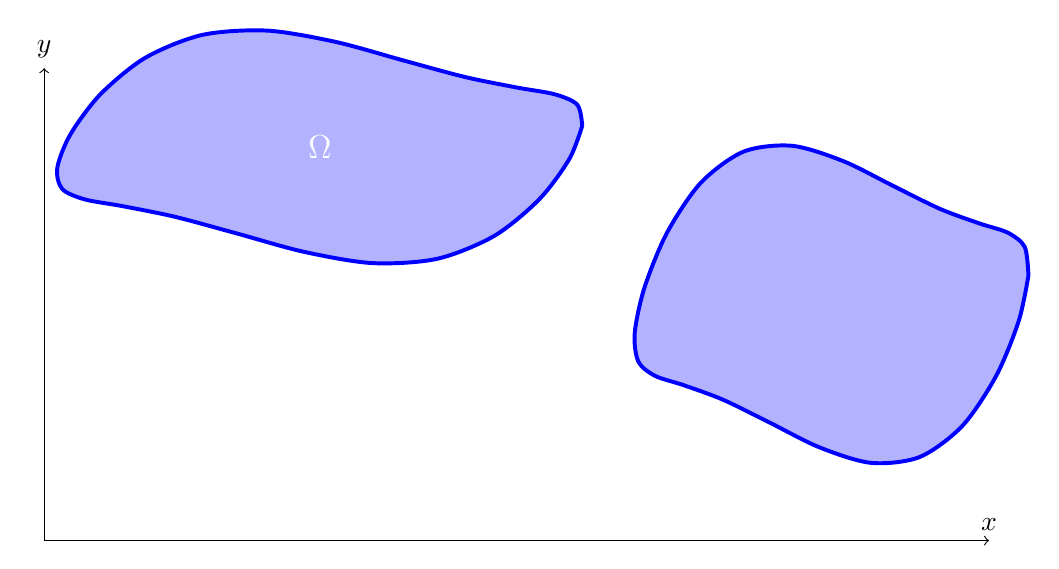
\begin{tikzpicture}[
        mdomain/.style = {blue, line width = 0.5mm, fill = blue, fill opacity = 0.3}
    ]
        \draw[mdomain] plot[smooth, variable=\u, domain=0:360]({(5 * cos(\u) + 0.3 * sin(\u))/1.5 + 3.5},{(2 * sin(\u) + 0.4 * cos(3 *\u))/1.5+5});
        \draw[mdomain] plot[smooth, variable=\u, domain=0:360, blue, thick, fill = blue, fill opacity = 0.6]({(5 * cos(\u) + 0.3 * sin(\u))/2 +10},{(2 * sin(\u) + 0.4 * cos(3 *\u))/1.1+3});

        \node[white] (A) at (3.5,5) {\large $\Omega$};

        \draw[->] (0,0) -- (12,0) node[above]{$x$};
        \draw[->] (0,0) -- (0,6) node[above]{$y$};
    \end{tikzpicture}
    \label{fig:deslocamento}
\end{figure}